\documentclass[conference]{IEEEtran}
\IEEEoverridecommandlockouts
\usepackage{cite}
\usepackage{amsmath,amssymb,amsfonts}
\usepackage{algorithmic}
\usepackage{graphicx}
\usepackage{textcomp}
\usepackage[table,xcdraw]{xcolor}
\usepackage{booktabs}
\usepackage{tabularx}
\usepackage{hyperref} 
\usepackage[linesnumbered, vlined]{algorithm2e}
\usepackage{float}
\usepackage{amsmath}
\usepackage{pgfplots}
\usepackage{natbib}
\pgfplotsset{compat=1.17}
\pagestyle{plain}

\def\BibTeX{{\rm B\kern-.05em{\sc i\kern-.025em b}\kern-.08em
    T\kern-.1667em\lower.7ex\hbox{E}\kern-.125emX}}


\begin{document}

\title{Advancement in Anti-Corruption Measures: Crafting a K-means Clustering-Based Algorithm for Enhanced Detection of Corruption Patterns}

\author{
  \IEEEauthorblockN{Nishat Tasnim}
  \IEEEauthorblockA{\textit{Department of Computer} \\ {Science and Engineering} \\
    \textit{University of Asia Pacific}\\
    Dhaka, Bangladesh \\
    \textit{Email: \href{mailto:21201149@uap-bd.edu}{21201149@uap-bd.edu}}}
  \and
  \IEEEauthorblockN{Nahida Afrin}
  \IEEEauthorblockA{\textit{Department of Computer} \\ {Science and Engineering} \\
    \textit{University of Asia Pacific}\\
    Dhaka, Bangladesh \\
    \textit{Email: \href{mailto:21201011@uap-bd.edu}{21201011@uap-bd.edu}}}
  \and
  \IEEEauthorblockN{Samira Afsana}
  \IEEEauthorblockA{\textit{Department of Computer} \\ {Science and Engineering} \\
    \textit{University of Asia Pacific}\\
    Dhaka, Bangladesh \\
    \textit{Email: \href{mailto:21201013@uap-bd.edu}{21201013@uap-bd.edu}}}
}

\maketitle

\vspace{-20pt}

\begin{abstract}
Addressing the persistent issue of corruption in Bangladesh, this paper endeavors to tackle the challenge of detecting corruption, particularly those instances that directly impact the general populace originating from governmental or organizational sources. We propose a novel algorithm that integrates data mining techniques to identify corrupt practices. The core of our approach involves the development of an intelligent system, incorporating a user evaluation interface. When individuals avail themselves of services from an organization, they have the opportunity to anonymously submit their opinions regarding specific individuals or organizations. Subsequently, a refined K-means clustering algorithm is employed to analyze the data, and the output is organized to rank individuals or organizations based on their corruption levels.
\end{abstract}

\vspace{8pt}

\begin{IEEEkeywords}
    corruption; data-mining; clustering; k-means
\end{IEEEkeywords}

\section{Introduction}
Corruption, defined as "the abuse of entrusted power for private gain," encompasses various forms such as grand, petty, and political, depending on the magnitude of money involved and the sector affected \cite{ref1}. Examples of corruption include bribery, embezzlement, fraud, extortion, conflict of interests, favoritism, nepotism, cronyism, and political corruption \cite{ref2}. Detection of corruption is particularly crucial in setups where a service provider directly interacts with their service receiver. Certain sectors bear a disproportionate impact of corruption, including public services, land administration, tax administration, customs administration, public procurement, the judicial system, law enforcement, banking, health services, and transportation \cite{ref3}. This paper proposes a model incorporating a modified K-means algorithm to determine the corruption level of an organization and the individuals involved. Opinions from service receivers and employees are stored in a database. The proposed algorithm, integrating data mining techniques, facilitates the creation of distinct groups and clusters based on the corruption levels of individuals. Clustering involves identifying similarities among data based on characteristics found in raw data \cite{ref4}. The term "clustering" is widely used in various research communities as a technique for grouping unlabeled data \cite{ref5}. The clustering process is continuous and iterative, contributing to knowledge discovery from vast quantities of raw and unorganized data \cite{ref6}. This concept can be applied in suggestion and complaint portals \cite{ref7}, ratings and reviews systems in e-commerce \cite{ref8}, online services \cite{ref9}, and teaching evaluation report systems \cite{ref10}.

\section{PROPOSED MODEL AND ALGORITHM}
\subsection{Proposed Model to Detect Corruption}
After receiving a service, the service receiver will receive login credentials via email. Subsequently, users are required to visit the evaluation portal to provide their opinions anonymously. Similarly, opinions are solicited from internal employees of the service provider. All collected opinions are stored in a database. Upon executing the proposed algorithm, the output will be generated. This result is sorted using the "Static Centroid K-means Clustering" to obtain the final result. The proposed model for detecting corruption is illustrated in Fig.~\ref{fig:model}.

\begin{figure}[h]
  \centering
  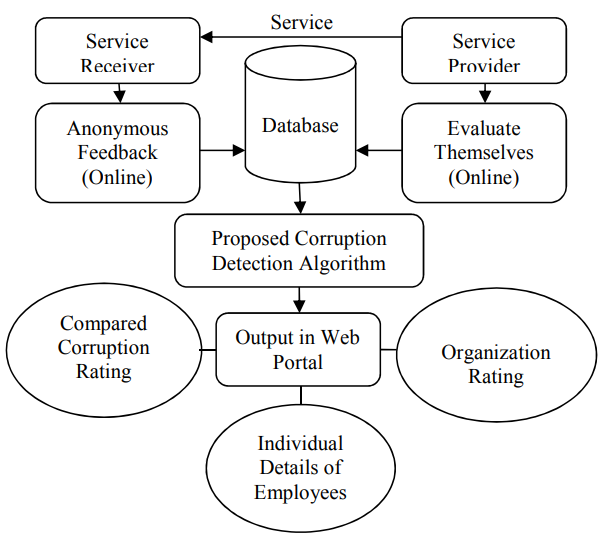
\includegraphics[width=0.5\linewidth]{corruption.png}
  \caption{Proposed Model to Detect Corruption.}
  \label{fig:model}
\end{figure}

\subsection{Proposed Algorithm}
The proposed \emph{Corruption Detection Algorithm} is a combination of the \emph{Proposed Algorithm} and \emph{Proposed Static Centroid K-means clustering} (Fig. ~\ref{fig:k-means-algorithm}), which is a modified version of the traditional K-means clustering \cite{ref11}. The \emph{Proposed Algorithm} utilizes the \emph{Proposed Static Centroid K-means clustering} to categorize the corrupted employees of an organization. The conventional K-means clustering algorithm has been modified compared to Hierarchical Clustering or Density-based Clustering algorithms to maintain the centroid as static. Hierarchical Clustering does not assume a specific number of clusters, and Density-based Clustering has a dynamic centroid. The proposed algorithm (Fig.~\ref{algorithm}) has been designed to detect corruption. This Corruption Detection Algorithm will be applied to both service receivers' opinions and the evaluation of employees themselves.

\begin{figure}[h]
  \centering
  \fbox{
    \begin{minipage}{0.9\linewidth}
      \begin{algorithm} [H]
      \LinesNumbered
      \textbf{Input:} $X = \{S_1, S_2, \ldots, S_K\}$\;
      
      \textbf{Determine:} \textit{upper and lower limit of X}\;
      
      \textbf{Count:} \textit{number of users} $N$\;
      
      \textbf{Average:} $f(z) = \sum_{n=0}^k \frac{X^n}{N}$\;
      
      \If{X \textit{contains maximum or minimum value}}
      {
          reject\;
      }
      \Else 
      {
          \textit{input the value to the database}\;
      }
      
      \textbf{Output:}
      
      \If{50 or fewer data sets}
      {
          \textit{execute static centroid k-means}\;
      }
      \Else
      {
          \textit{delete older date} then \textit{execute static centroid k-means}\;
      }
      \end{algorithm}
    \end{minipage}
  }
  \caption{Proposed Corruption Detection Algorithm}
  \label{algorithm}
\end{figure}

The flowchart of the proposed algorithm is depicted in Fig.~\ref{fig:flowchart}.

\begin{figure}[h]
  \centering
  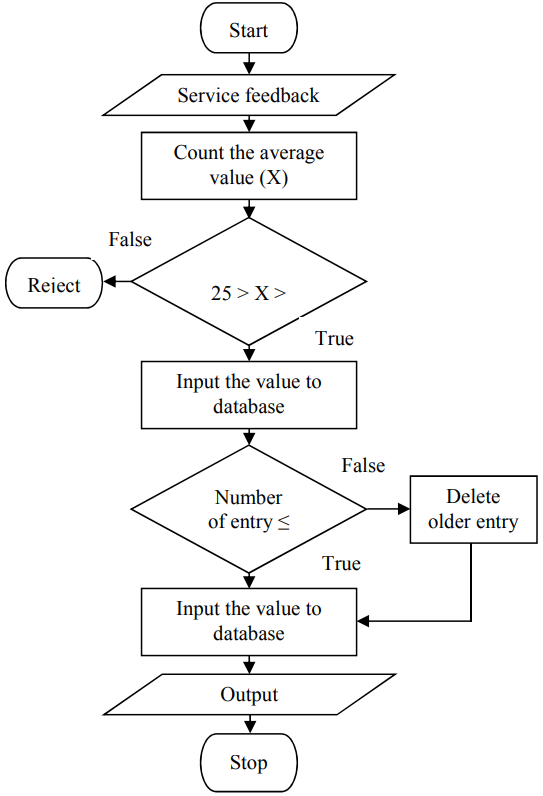
\includegraphics[width=0.5\linewidth]{flowchart.png}
  \caption{Flowchart of the proposed algorithm.}
  \label{fig:flowchart}
\end{figure}

When the service receiver visits the evaluation portal to provide their opinion, the algorithm starts executing through a web server. The service receiver sees only those employees' names on the evaluation interface who are directly involved in the service. To address potential knowledge gaps about indirectly involved employees, a tracking server is employed, and employees must log in with their individual credentials. The server traces the list of employees who served a specific service receiver. Consequently, the evaluation portal displays only those employees who directly provided the service. The service receiver then selects employees one by one and evaluates them using a form that includes 5 psychological statements related to honesty, professionalism, helpfulness, etc. Each statement offers 5 options (strongly disagree, disagree, neutral, agree, strongly agree), each assigned points from 1 to 5. The points range from 5 to 25, and the average points are calculated. To avoid extreme values (maximum and minimum points), the algorithm filters them.

\subsection{Proposed Static Centroid K-means Clustering Algorithm}

Static Centroid K-means clustering is almost similar to the traditional \textit{K-means Clustering}. The traditional K-means algorithm is based on a simple idea: Given a set of initial clusters, assign each point to one of them, then each cluster center is replaced by the mean point on the respective cluster \cite{ref12}. For the proposed fixed centroid K-means clustering, the difference is that the centroid value is defined manually, and it will be static for all the centers. The proposed static centroid K-means clustering is shown in Fig.~\ref{fig:static-k-means}.

\begin{figure}[h]
  \centering
    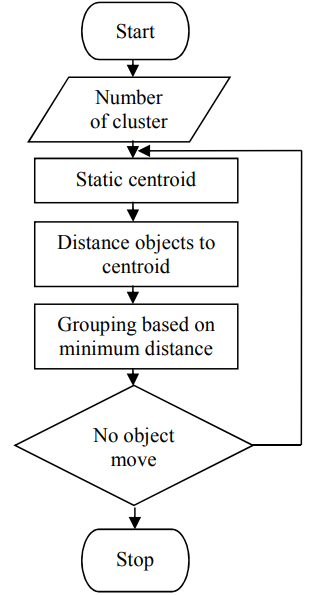
\includegraphics[width=0.35\linewidth]{flowchart1.png}
  \caption{Flowchart of the proposed static centroid K-means algorithm.}
  \label{fig:static-k-means}
\end{figure}

Here is the algorithm for the proposed static centroid K-means clustering in Fig.~\ref{fig:k-means-algorithm}.

\begin{figure}[h]
  \centering
  \fbox{
    \begin{minipage}{0.9\linewidth}
      \begin{algorithm}[H]
      \LinesNumbered
      \textbf{Select static K cluster centroids} $\mu_{1}, \mu_{2}, \ldots, \mu_{K} \in \mathbb{R}$\;
      
      \Repeat{for $i = 1$ to $m$}{
        $c^{(i)} =$ index (from 1 to $K$) of cluster centroid closest to $X^{(i)}$\;
        \For{$k = 1$ to $K$}{
          $\mu_{K} =$ average (mean) of points assigned to cluster $k$\;
        }
      }
      \end{algorithm}
    \end{minipage}
  }
  \caption{Proposed static centroid K-means algorithm.}
  \label{fig:k-means-algorithm}
\end{figure}

\section{Datasets and Experiments}

\subsection{Experiment with Test Dataset}

In this section, we present an experiment conducted with a 2-dimensional dataset. The x-axis represents the sum of average points from internal employees, while the y-axis represents the sum of average points from service receivers. The objective is to detect corruption for an employee named "A." The x-values are taken from Table~\ref{tab:table2}, and the y-values are taken from Table~\ref{tab:table1}. Other employees' scores are assumed as a test dataset from Table~\ref{tab:table3}.
\vspace{10pt}

\renewcommand{\arraystretch}{1.9}
\begin{table}[H]
  \centering
  \begin{tabularx}{\linewidth}{|c|*{5}{X|}}
    \hline
    \rowcolor[HTML]{EFEFEF}
    \multicolumn{6}{c}{\cellcolor[HTML]{EFEFEF}{\color[HTML]{000000} \textbf{TABLE I. POINTS FROM SERVICE RECEIVER}}}\\ \hline
    Service Receiver  & Q. 1 & Q. 2 & Q. 3 & Q. 4 & Q. 5 \\ \hline
    Person 1          & 4    & 5    & 3    & 4    & 2    \\ \hline
    Person 2          & 5    & 4    & 3    & 5    & 3    \\ \hline
    Person 3          & 4    & 5    & 5    & 5    & 4    \\ \hline
    Average Points    & 4.3  & 4.7  & 3.3  & 4.7  & 3    \\ \hline
  \end{tabularx}
  \caption{}
  \label{tab:table1}
\end{table}

\vspace{-18pt}

\begin{table}[H]
  \centering
  \begin{tabularx}{\linewidth}{|c|*{5}{X|}}
    \hline
    \rowcolor[HTML]{EFEFEF}
    \multicolumn{6}{c}{\cellcolor[HTML]{EFEFEF}{\color[HTML]{000000} \textbf{TABLE II. POINTS FROM EMPLOYEES}}}\\ \hline
    Employees          & Q. 1 & Q. 2 & Q. 3 & Q. 4 & Q. 5 \\ \hline
    Person 1           & 5    & 5    & 4    & 4    & 5    \\ \hline
    Person 2           & 5    & 4    & 5    & 5    & 3    \\ \hline
    Person 3           & 4    & 5    & 4    & 5    & 4    \\ \hline
    Average Points     & 4.7  & 4.7  & 4.3  & 4.7  & 4    \\ \hline
  \end{tabularx}
  \caption{}
  \label{tab:table2}
\end{table}

\vspace{-18pt}

\begin{table}[H]
  \centering
  \begin{tabularx}{\linewidth}{|c|*{2}{X|X|}}
    \hline
    \rowcolor[HTML]{EFEFEF}
    \multicolumn{3}{c}{\cellcolor[HTML]{EFEFEF}{\color[HTML]{000000} \textbf{TABLE III. SUM OF AVERAGES}}}\\ \hline
    Employee Name       & \begin{tabular}[c]{@{}c@{}}Sum of Average Points \\ (From Employees)\end{tabular} & \begin{tabular}[c]{@{}c@{}}Sum of Average Points\\ (From Service Receiver)\end{tabular} \\ \hline
    A                   & 22.3 & 20 \\ \hline
    B                   & 24.3 & 23.4 \\ \hline
    C                   & 18.5 & 17.5 \\ \hline
    D                   & 17.3 & 18.2 \\ \hline
    E                   & 10.8 & 7.6  \\ \hline
    F                   & 18.6 & 14.3 \\ \hline
    G                   & 20.4 & 19.5 \\ \hline
    H                   & 17.2 & 22.8 \\ \hline
    I                   & 20.7 & 21.6 \\ \hline
    J                   & 12.7 & 14.3 \\ \hline
    K                   & 15.5 & 16   \\ \hline
    L                   & 16.7 & 17.5 \\ \hline
  \end{tabularx}
  \caption{}
  \vspace{-18pt} 
  \label{tab:table3}
\end{table}

Corruption score of employees is shown in Fig.~\ref{fig:corruption_score} which is drawn from Table~\ref{tab:table3}.

\begin{figure}[H]
  \centering
  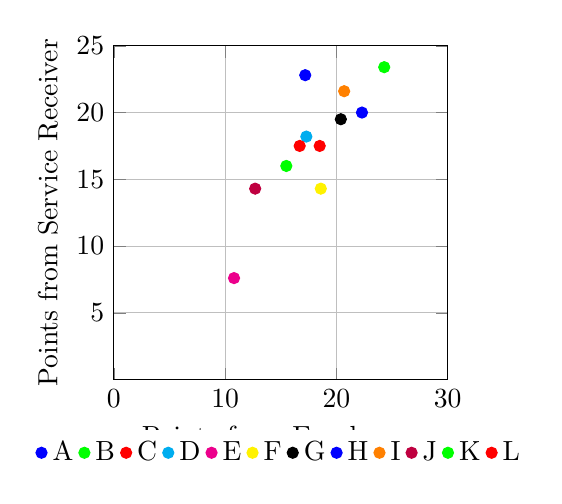
\begin{tikzpicture}
    \begin{axis}[
      width=0.48\textwidth,
      height=0.48\textwidth,
      xlabel={Points from Employees},
      ylabel={Points from Service Receiver},
      legend pos=north west, grid=major,
      xtick={0, 10, 20, 30},
      ytick={5, 10, 15, 20, 25},
      xmin=0, xmax=30, ymin=0, ymax=25,
      legend image post style={mark=*},
      legend entries={A, B, C, D, E, F, G, H, I, J, K, L},
      legend style={legend columns=-1, cells={anchor=west}, at={(0.5,-0.15)}, anchor=north, draw=none}
    ]
      \addplot[scatter, only marks,
        scatter src=explicit symbolic,
        scatter/classes={
            a={mark=*,blue}, b={mark=*,green}, c={mark=*,red}, d={mark=*,cyan}, e={mark=*,magenta}, f={mark=*,yellow}, 
            g={mark=*,black}, h={mark=*,blue}, i={mark=*,orange}, j={mark=*,purple}, k={mark=*,green}, l={mark=*,red}
        }]
      table[meta=label] {
        x y label
        22.3 20 a
        24.3 23.4 b
        18.5 17.5 c
        17.3 18.2 d
        10.8 7.6 e
        18.6 14.3 f
        20.4 19.5 g
        17.2 22.8 h
        20.7 21.6 i
        12.7 14.3 j
        15.5 16 k
        16.7 17.5 l
      };
    \end{axis}
  \end{tikzpicture}
  \vspace{-10pt}
  \caption{Two-dimensional corruption score of employees.}
  \label{fig:corruption_score}
\end{figure}
\renewcommand{\arraystretch}{1.0}

Before calculating static centroid K-means clustering, we will execute traditional K-means clustering. For traditional K-means clustering, we can use the Sum of Squared Error (SSE). It calculates the Euclidean distance to the nearest centroid and computes the total sum of the squared errors. The different sets of clusters which are produced on different runs of K-means, we consider the one with the smallest squared errors \cite{ref13}. The SSE is defined as follows:

\begin{equation}
    arg \underset{c}{min} \sum_{i=1}^{k} \sum_{x \in c_i}^{} d(x,\mu _i)= arg \underset{c}{min} \sum_{i=1}^{k} \sum_{x \in c_i}^{} \left\| x-\mu_i \right\|_{2}^{2}
\end{equation}

\vspace{10pt}

Where, \(c_i\) is the set of points that belong to cluster \(i\). The K-means clustering uses the square of the Euclidean distance \cite{ref9}. After calculating, we get three clusters and the final centroids value which is shown in Table \ref{tab:centroids}.

\vspace{10pt}

\renewcommand{\arraystretch}{2}
\begin{table}[H]
  \centering
  \begin{tabular}{cccc}
    \hline
    \multicolumn{4}{c}{\cellcolor[HTML]{EFEFEF}{\color[HTML]{000000} \textbf{TABLE IV. INITIAL AND FINAL CENTERS}}} \\ \hline
    \multicolumn{1}{|c|}{Cluster} & \multicolumn{1}{c|}{Employee} & \multicolumn{1}{c|}{Initial Centroid} & \multicolumn{1}{c|}{Final Centroid} \\ \hline
    \multicolumn{1}{|c|}{1} & \multicolumn{1}{c|}{A,B,C,D,F,G,H,I,K,L} & \multicolumn{1}{c|}{21,21} & \multicolumn{1}{c|}{19.9,19.6} \\ \hline
    \multicolumn{1}{|c|}{2} & \multicolumn{1}{c|}{J} & \multicolumn{1}{c|}{14.5,14.5} & \multicolumn{1}{c|}{12.7,14.3} \\ \hline
    \multicolumn{1}{|c|}{3} & \multicolumn{1}{c|}{E} & \multicolumn{1}{c|}{8.5,8.5} & \multicolumn{1}{c|}{10.8,7.6} \\ \hline
  \end{tabular}
  \vspace{8pt}
  \caption{}
  \label{tab:centroids}
\end{table}

So, from the traditional K-means clustering, we get the following three clusters (Fig.~\ref{fig:clusters}).

\begin{figure}[h]
    \centering
    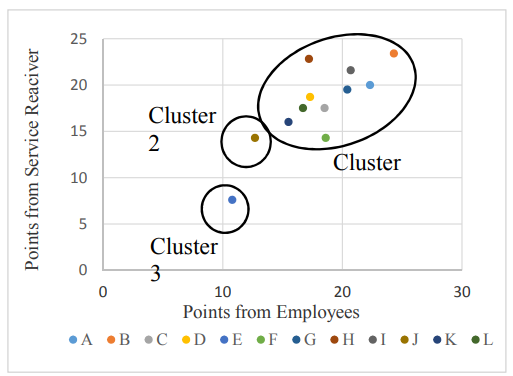
\includegraphics[width=0.4\textwidth]{cluster1.png}
    \caption{Three clusters by using traditional K-means algorithm.}
    \label{fig:clusters}
\end{figure}

Now, we will execute the proposed static centroid K-means algorithm. For this algorithm, we will calculate the distance from all the values (employee’s corruption score) to three static centroids. Then we will select the minimum distance for the appropriate cluster. Where, distance, \(D\) is defined as follows,

\begin{equation}
    D = \sqrt{(x_{1}- x_{2})^{2} + (y_{1}- y_{2})^{2}}
\end{equation}

According to our proposed algorithm, the corruption score (\(X\)) will be greater than 5 and less than 25, so we have considered three centroids as \(C1 (21, 21)\), \(C2 (14.5, 14.5)\), \(C3 (8.5, 8.5)\) to split the employees into three clusters. In case of the same distance, we have chosen the distance from the greater centroid (i.e. Score of employee D). The distance from all the employee’s corruption score to three static centroids is shown in Table \ref{tab:distance}.

\vspace{8pt}

\renewcommand{\arraystretch}{1.6}
\begin{table}[H]
    \centering
    \begin{tabular}{ccccc}
        \hline
        \multicolumn{5}{c}{\cellcolor[HTML]{EFEFEF}{\color[HTML]{000000} \textbf{     TABLE V.    DISTANCE FROM THREE CENTROID    }}} \\ \hline
        \multicolumn{1}{|c|}{\begin{tabular}[c]{@{}c@{}}Score of\\ Employees\end{tabular}} & 
        \multicolumn{1}{c|}{\begin{tabular}[c]{@{}c@{}}Distance \\ From C1\end{tabular}} & 
        \multicolumn{1}{c|}{\begin{tabular}[c]{@{}c@{}}Distance \\ From C2\end{tabular}} & 
        \multicolumn{1}{c|}{\begin{tabular}[c]{@{}c@{}}Distance \\ From C3\end{tabular}} & 
        \multicolumn{1}{c|}{Cluster} \\ \hline
        \multicolumn{1}{|c|}{A(22.3, 20)} & \multicolumn{1}{c|}{1.64} & \multicolumn{1}{c|}{9.54} & \multicolumn{1}{c|}{17.96} & \multicolumn{1}{c|}{1} \\ \hline
        \multicolumn{1}{|c|}{B(24.3, 23.4)} & \multicolumn{1}{c|}{4.08} & \multicolumn{1}{c|}{13.23} & \multicolumn{1}{c|}{21.71} & \multicolumn{1}{c|}{1} \\ \hline
        \multicolumn{1}{|c|}{C(18.5, 17.5)} & \multicolumn{1}{c|}{4.30} & \multicolumn{1}{c|}{5.00} & \multicolumn{1}{c|}{13.45} & \multicolumn{1}{c|}{1} \\ \hline
        \multicolumn{1}{|c|}{D(17.3, 18.2)} & \multicolumn{1}{c|}{4.64} & \multicolumn{1}{c|}{4.64} & \multicolumn{1}{c|}{13.09} & \multicolumn{1}{c|}{1} \\ \hline
        \multicolumn{1}{|c|}{E(10.8, 7.6)} & \multicolumn{1}{c|}{16.84} & \multicolumn{1}{c|}{7.82} & \multicolumn{1}{c|}{2.46} & \multicolumn{1}{c|}{3} \\ \hline
        \multicolumn{1}{|c|}{F(18.6, 14.3)} & \multicolumn{1}{c|}{7.11} & \multicolumn{1}{c|}{4.10} & \multicolumn{1}{c|}{11.64} & \multicolumn{1}{c|}{2} \\ \hline
        \multicolumn{1}{|c|}{G(20.4, 19.5)} & \multicolumn{1}{c|}{1.61} & \multicolumn{1}{c|}{7.73} & \multicolumn{1}{c|}{16.20} & \multicolumn{1}{c|}{1} \\ \hline
        \multicolumn{1}{|c|}{H(17.2, 22.8)} & \multicolumn{1}{c|}{4.20} & \multicolumn{1}{c|}{8.72} & \multicolumn{1}{c|}{16.73} & \multicolumn{1}{c|}{1} \\ \hline
        \multicolumn{1}{|c|}{I(20.7, 21.6)} & \multicolumn{1}{c|}{0.67} & \multicolumn{1}{c|}{9.42} & \multicolumn{1}{c|}{17.90} & \multicolumn{1}{c|}{1} \\ \hline
        \multicolumn{1}{|c|}{J(12.7, 14.3)} & \multicolumn{1}{c|}{10.66} & \multicolumn{1}{c|}{1.81} & \multicolumn{1}{c|}{7.16} & \multicolumn{1}{c|}{2} \\ \hline
        \multicolumn{1}{|c|}{K(15.5, 16)} & \multicolumn{1}{c|}{7.43} & \multicolumn{1}{c|}{1.80} & \multicolumn{1}{c|}{10.25} & \multicolumn{1}{c|}{2} \\ \hline
        \multicolumn{1}{|c|}{L(16.7, 17.5)} & \multicolumn{1}{c|}{5.54} & \multicolumn{1}{c|}{3.72} & \multicolumn{1}{c|}{12.17} & \multicolumn{1}{c|}{2} \\ \hline
    \end{tabular}
    \vspace{8pt}
    \caption{}
    \label{tab:distance}
\end{table}

Cluster 1 is for the group of honest people. Cluster 2 is for average (less honest) persons, and Cluster 3 is for the corrupted employee’s group. So, we get different three clusters from the proposed static centroid K-means algorithm, as shown in Fig. \ref{fig:clusters}.

\begin{figure}[H]
    \centering
    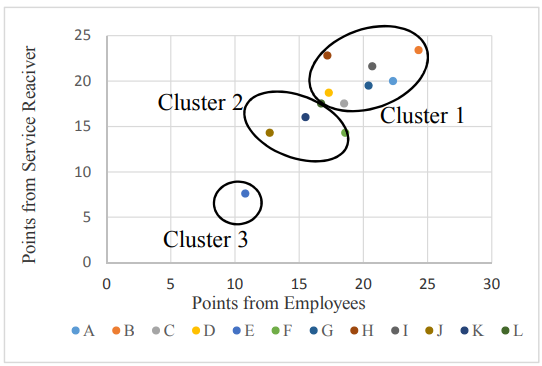
\includegraphics[width=0.45\textwidth]{cluster2.png}
    \caption{Three clusters by using static centroid K-means algorithm.}
    \label{fig:cluster2}
\end{figure}

\subsection{Result Analysis}

We can see from Fig. \ref{fig:clusters} that, for traditional K-means clustering where the density of data is high, a single large cluster (Cluster 1) has been created. In this situation, some lower values (i.e., F, K, and L) are in Cluster 1 as well as in the group of honest people, though they are average in corruption rating. We can solve this problem by using the proposed static centroid K-means clustering algorithm. According to this algorithm, centroids will be static. So, the lower value will not be an element of the upper cluster, and the upper value will not be an element of the lower cluster as well. We can see from Fig. \ref{fig:cluster2} that the average corruption ratings are in Cluster 1, higher corruption ratings are in Cluster 2, and the lower ones are in Cluster 3 as well.

\section{Conclusion and Challenges}

There is a lot of future scope for this model. The proposed model can be enhanced by adding a comment \& multimedia attachment option, a public opinions field in the output page, etc. An auto mail sending option to concern organizations for a specific time duration can be developed. It is possible to generate a history graph to find the state of the corruption. The model will be capable of data synchronization for the transfer issue and synchronized with an SMS-based evaluation system. This algorithm can be applied as a digital complaint and suggestion box. Nevertheless, there are some limitations to this online-based idea. The main challenge of this system is that people need the Internet everywhere in the country. Finally, this model will be useful in society if the corrupted people are being faced with punishment. It is also needed to make awareness against corruption and its awful effect. Education from the family can be more effective to increase morality.

% Reference:

\bibliographystyle{ieeetr}

\begin{thebibliography}{99}

\bibitem{ref1}
Transparency International. (2018). What is Corruption? Retrieved from \url{https://www.transparency.org/what-is-corruption}

\bibitem{ref2}
Assignment Point. (2018). Corruption in Bangladesh. Retrieved from \url{www.assignmentpoint.com/arts/social-science/corruption-bangladesh}

\bibitem{ref3}
Bliss, B. (2018). Bangladesh Corruption Report. Business Anti-Corruption Portal. Retrieved from \url{https://www.business-anti-corruption.com/country-profiles/bangladesh/}

\bibitem{ref4}
I.S. Dhillon and D.M. Modha, “Concept decompositions for large sparse text data using clustering,” Machine Learning, vol. 42, issue 1, pp. 143-175, 2001.

\bibitem{ref5}
C.C. Aggarwal, J. Han, J. Wang, and P.S. Yu, "A framework for projected clustering of high dimensional data streams" in Proceedings of the Thirtieth international conference on Very large databases-Vol 30, 2004, p. 863.

\bibitem{ref6}
T. Kanungo, D. M. Mount, N. S. Netanyahu, C. D. Piatko, R. Silverman, and A. Y. Wu, “An efficient K-means clustering algorithm,” IEEE Trans. Pattern Analysis and Machine Intelligence, vol. 24, pp. 881-892, 2002.

\bibitem{ref7}
Just.edu.jo. (2018). Complaints and suggestion system. Retrieved from \url{http://www.just.edu.jo/Centers/HealthCenter/Pages/Complaints-and-suggestion-system.aspx}

\vspace{350pt}

\bibitem{ref8}
Online Shipping Blog | Endicia. (2018). Customer Feedback and Why Your E-commerce Store Needs It - Online Shipping Blog | Endicia. Retrieved from \url{https://online-shipping-blog.endicia.com/customer-feedback-and-why-your-e-commerce-store-needs-it/}

\bibitem{ref9}
Team, L., Directors, B., News, P., Us, C., Programs, S. and Videos, A. (2018). How You Can Use Customer Feedback to Improve Your Business - Insightly. Retrieved from \url{https://www.insightly.com/blog/how-you-can-use-customer-feedback-to-improve-your-business/}

\bibitem{ref10}
Asd.k12.pa.us. (2018). Teacher Evaluation – Staff – Armstrong School District. Retrieved from \url{https://www.asd.k12.pa.us/apps/pages/index.jsp?uREC_ID=417164&type=d&pREC_ID=912373}

\bibitem{ref11}
P. Tan, M. Steinbach, A. Karpatne and V. Kumar, Introduction to data mining. New York, NY: Pearson Education, 2018.

\bibitem{ref12}
Shi Na, Liu Xumin, “Research on K-means Clustering Algorithm”, IEEE Third International Conference on Intelligent Information Technology and Security Informatics, 2010.

\bibitem{ref13}
H. Gonçalves, "K-means clustering - algorithm and examples", Onmyphd.com, 2018. Retrieved from \url{https://www.onmyphd.com/?p=k-means.clustering}

\end{thebibliography}

\end{document}

%THE END! BYE!